\chapter{Rouge}
\begin{quotation}
\textsl{You are a nameless traveller that has been compelled to search for something. An object, a person, or just a place. You don't know yet, but it's up to you to find out. You will travel through various caves, forests and towns to pursue the whims of your heart. Every time you seem to solve a problem, another one turns up. Always moving you towards some inevitable doom. Are you born for heroism, or will you die unloved and unknown? \\\\Choose your path, and see where the voices in your head take you.}
\end{quotation}
Rouge is a \rogue tile-based game that is created specifically for the demonstration of the \diage narrative generation system. Created within my own framework \textit{SilicaLib} created on top of the XNA game-framework created by Microsoft. Rouge is characterised by the fact that the world and the narrative is generated by the direct influence of the player.

\section{Mechanics}
In Rouge, the player moves through the world one tile at a time. 

\section{World generation}
The world within Rouge is procedurally generated by a cellular automaton. During a step of this automaton, the algorithm walks through the game world and checks each tile for certain conditions pertaining to their neighbours. If these conditions are met, his state will be changed accordingly. The states a tile has in Rouge are a simple \textit{alive} or \textit{dead} state. When a tile has 5 or more live neighbours, the tile becomes alive themselves. However, when a tile has less than 2 live neighbours, the tile dies. The first rule ensures that tiles group together, and the other rule destroys any singular 'island' tiles.

\begin{algorithm}
	\KwIn{tilemap}
	\KwOut{new tilemap}
	let \textit{deadCells} and \textit{liveCells} be an empty collection of tiles\;
	\ForEach{tile in tilemap}{
		\uIf{tile.neighbours $\geq$ 5}{
			liveCells.push(tile)\;
		}\uElseIf{tile.neighbours $\leq$ 1}{
			deadCells.push(tile)\;
		}
	}
	\ForEach{tile in deadCells}{
		tile.alive = false\;
	}
	\ForEach{tile in liveCells}{
		tile.alive = true\;
	}
	\caption{Cellular Automation algorithm as used in Rouge}\label{alg:ca}
\end{algorithm}

\begin{figure}
	\centering
	\begin{subfigure}[b]{0.3\textwidth}
		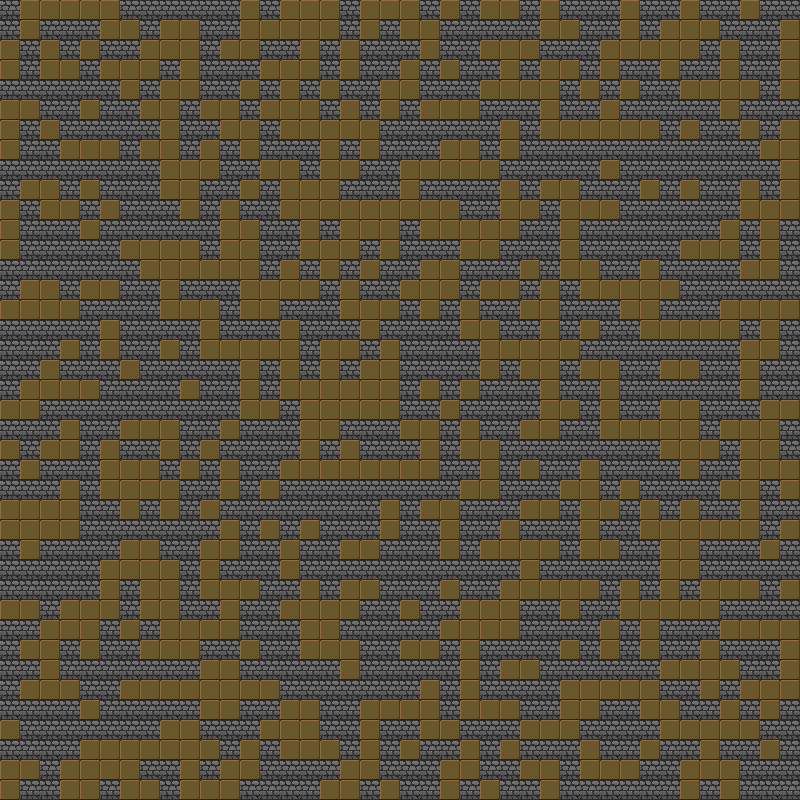
\includegraphics[width=\textwidth]{rouge/screenshot0}
		\caption{Initial map}
	\end{subfigure}	
	~
	\begin{subfigure}[b]{0.3\textwidth}
		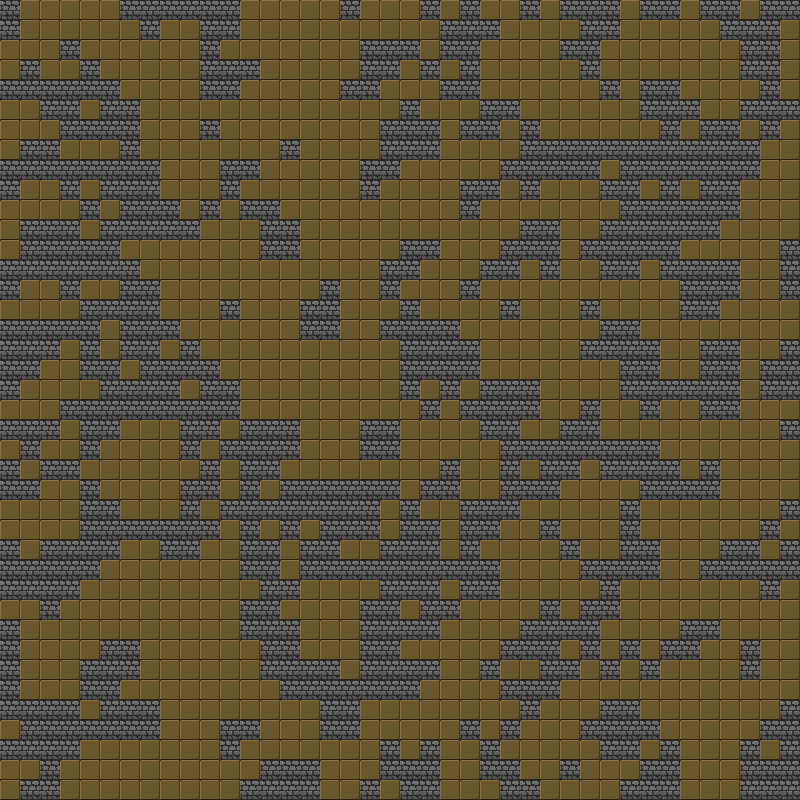
\includegraphics[width=\textwidth]{rouge/screenshot1}
		\caption{Step 1}
	\end{subfigure}	
	~
	\begin{subfigure}[b]{0.3\textwidth}
		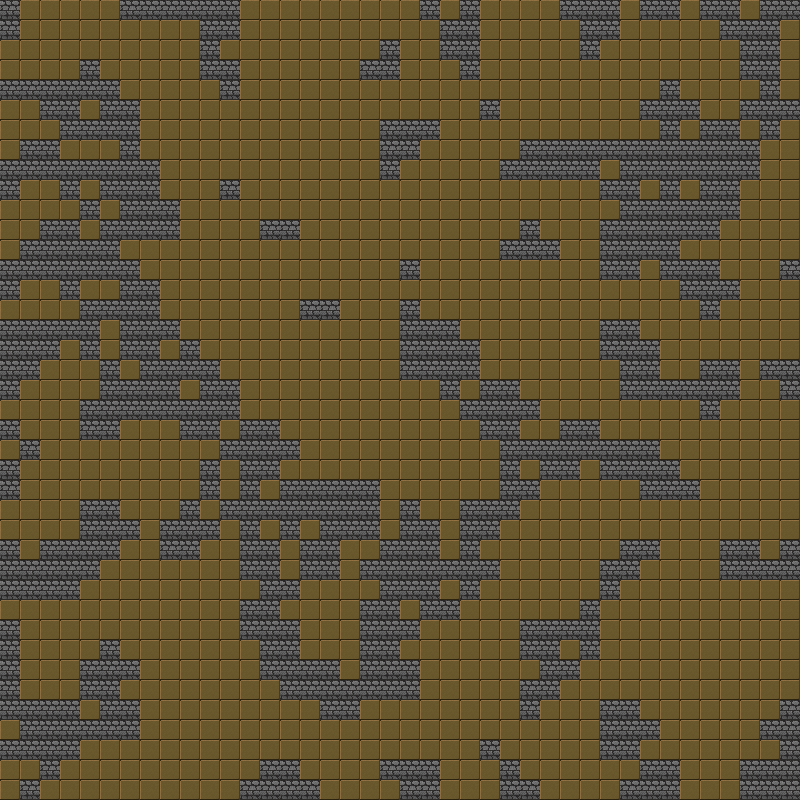
\includegraphics[width=\textwidth]{rouge/screenshot2}
		\caption{Step 2}
	\end{subfigure}	
	~
	\begin{subfigure}[b]{0.3\textwidth}
		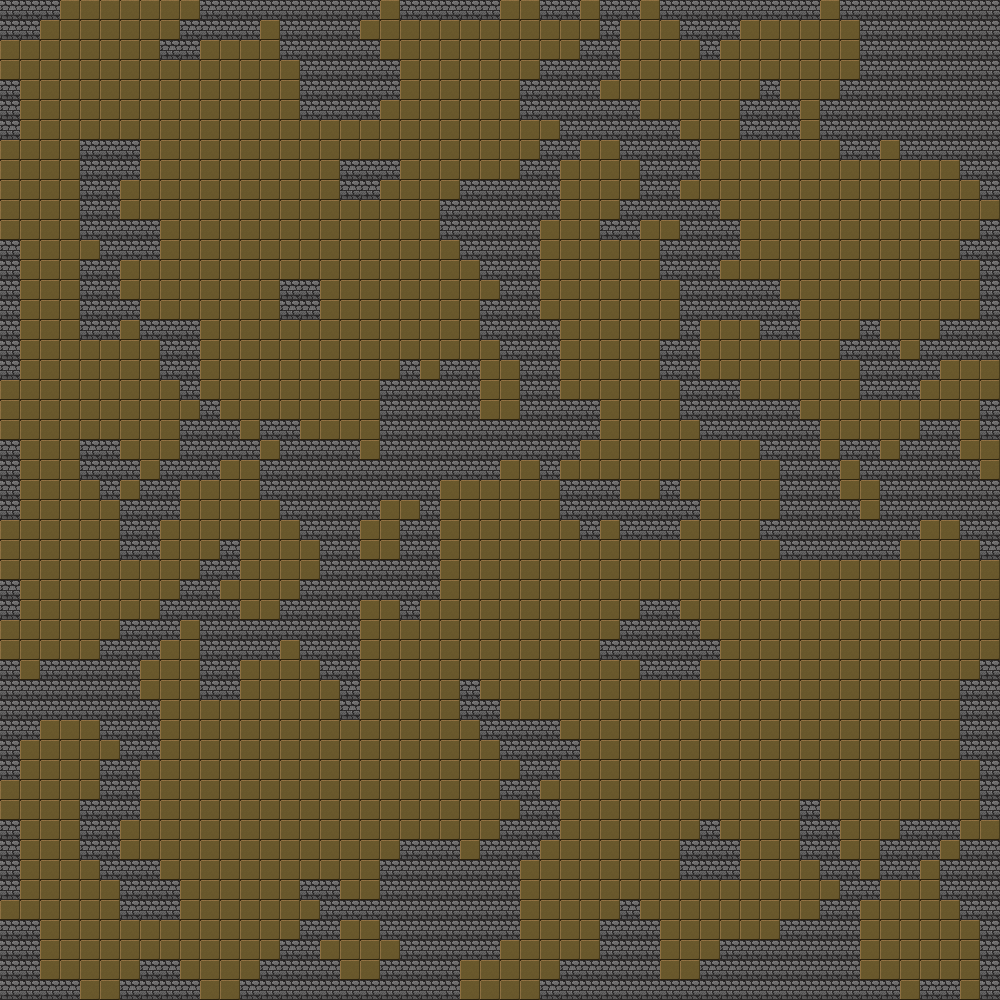
\includegraphics[width=\textwidth]{rouge/screenshot3}
		\caption{Step 3}
	\end{subfigure}		
	~
	\begin{subfigure}[b]{0.3\textwidth}
		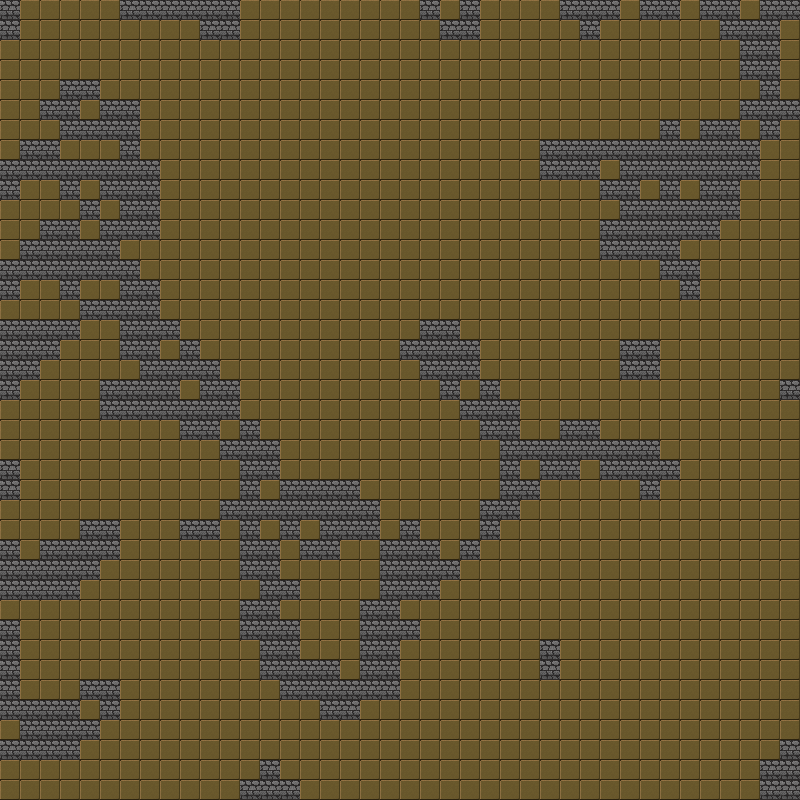
\includegraphics[width=\textwidth]{rouge/screenshot4}
		\caption{Step 4}
	\end{subfigure}
	~
	\begin{subfigure}[b]{0.3\textwidth}
		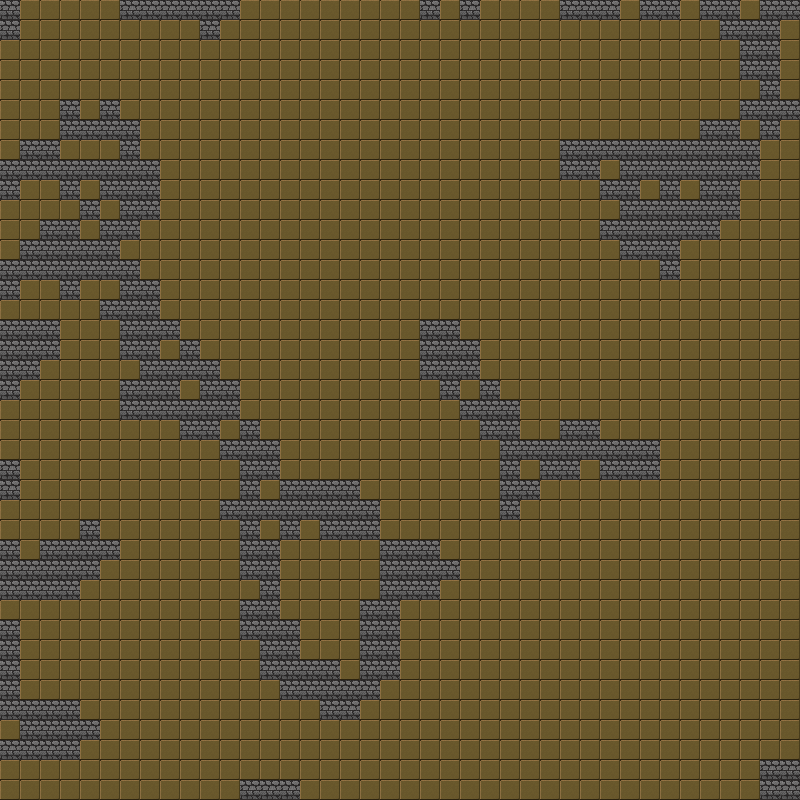
\includegraphics[width=\textwidth]{rouge/screenshot5}
		\caption{Step 5}
	\end{subfigure}	
	\caption{The generation of a 50 x 50 tilemap with 20 x 20 (pixels) tiles}\label{fig:rouge:screens}
\end{figure}